%% Capitol 2 - Descripció dels diferents components d'un sistema encastat: Microcontroladors, perifèrics, busos

\chapter{Breu introducció als sistemes encastats}
\label{ch:components}

Un sistema encastat és, bàsicament, un seguit de components hardware i software treballant conjuntament per obtenir una aplicació o funcionalitat determinada.

Els components hardware es poden dividir en tres grans blocs:
\begin{itemize}
\item procés de dades: dispositiu amb la capacitat de gestionar dades, entrada sortida, etc. Pot ser un microcontrolador, un \gls{DSP}, una \gls{FPGA}, un \gls{ASIC} o un sistema hibrid que incorpori varis dels anteriors dins el mateix hardware.
 \item sensors o introducció de dades. Qualsevol dispositiu que rep estímuls del mon físic i els converteix en dades, ja siguin digitals o analògiques (termòmetre, pantalla tàctil, acceleròmetre, etc.).
 \item actuadors o presentació de dades. Qualsevol dispositiu que rep una dada o sèrie de dades i ho converteix en una acció física (motor, pantalla, relé, etc.).
\end{itemize}


\section{Microcontroladors}
Un microcontrolador està compost bàsicament d'una \gls{CPU}, memòria \gls{RAM} i \gls{ROM}, i un seguit de perifèrics tot integrat en un sol dispositiu. La varietat de microcontroladors diferents que es poden trobar al mercat és ingent, fent impossible fer un llistat de totes les opcions disponibles.

Històricament cada fabricant de microcontroladors tenia les seves pròpies famílies de dispositius (amb la seva pròpia arquitectura) amb les eines necessàries i, habitualment, cada conjunt era diferent i incompatible amb els demès.
Durant els últims anys aquest panorama ha canviat força, ja que molts fabricants han acabat adoptant una sola arquitectura. Aquesta arquitectura és l'anomenada {\bf \gls{Cortex}} de l'empresa \gls{ARM} \cite{Cortex}. Els fabricants trien quin model de CPU volen incorporar al seu dispositiu i hi afegeixen els perifèrics del seu catàleg que consideren que cal a cada dispositiu concret. D'aquesta manera, un sol fabricant té desenes o centeners de dispositius diferents basats en una mateixa CPU i amb diferents combinacions i nombre de perifèrics i memòria.

Tot i que tenim diferents dispositius de diferents fabricants que poden tenir la mateixa CPU, un executable no serà compatible entre aquests dispositius, ja que, segurament, el mapa de memòria o els diferent perifèrics seran diferents i, per tant, incompatibles.

Alguns dels fabricants més reconeguts de microcontroladors actuals són els següents:
\begin{itemize}
 \item \acrfull{Silabs} \cite{SiLabs}
 \item \acrfull{TI} \cite{TI}
 \item \acrfull{NXP} \cite{NXP}
 \item \acrfull{ST} \cite{ST}
 \item Microchip, antiga Atmel \cite{Microchip}
\end{itemize}

\section{ARM Cortex}
\label{sec:cortex}
Com ja hem dit, l'arquitectura \gls{Cortex} és actualment una de les més esteses en el camp dels processadors i microcontroladors de 32 bits. Es presenten tres perfils diferents segons l'àmbit d'aplicació:
\begin{itemize}
 \item {\bf Cortex-A} (d'{\bf A}plicació) Processadors d'altes prestacions per usos en telèfons mòbils, servidors, {\em tablets}, etc. \cite{CortexA}.
 \item {\bf Cortex-R} (de Temps {\bf R}eal) Dissenyats per aplicacions amb alts requeriments de seguretat com dispositius mèdics, aviònica o \glspl{PLC} \cite{CortexR}.
 \item {\bf Cortex-M} (de {\bf M}icrocontrolador) CPUs dissenyats per microcontroladors i aplicacions de baix consum \cite{CortexM}.
\end{itemize}

En aquest llibre i curs ens centrarem exclusivament a parlar del Cortex-M i les seves versions.

\begin{figure}
 \centering
 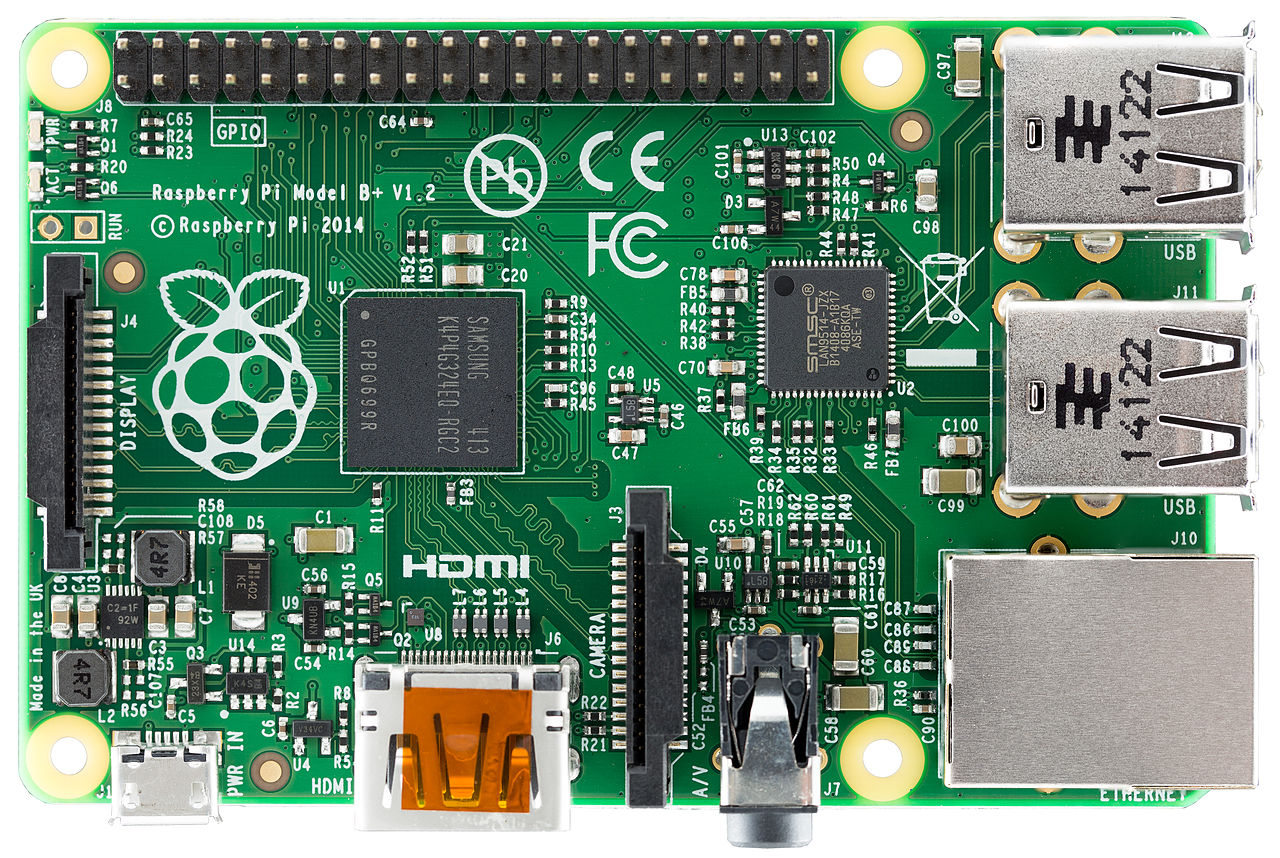
\includegraphics[width=0.65\textwidth, keepaspectratio]{imatges/Raspberry_Pi}
 \caption{Raspberry Pi amb un processador Cortex-A}{Raspberry Pi amb un processador Cortex-A. Per Lucasbosch [CC BY-SA 3.0], de la Wikimedia Commons \url{https://upload.wikimedia.org/wikipedia/commons/thumb/6/6f/Raspberry_Pi_B\%2B_top.jpg/512px-Raspberry_Pi_B\%2B_top.jpg}}
 \label{fig:Raspberry_Pi}
\end{figure}

\subsection{Cortex-M}
Aquesta arquitectura proposada per ARM és una arquitectura tipus RISC de 32 bits amb suport de {\em cache}, punt flotant i dissenyada per ser de baix consum. Tot i que hi ha diferents versions d'aquesta arquitectura, mantenen un conjunt d'instruccions comuns. Aquí llistem els més habituals \cite[7]{EmbeddedBook}:

\begin{itemize}
 \item {\bf Cortex-M0+}: És la versió més bàsica d'aquesta arquitectura, orientat a dispositius molt barats i senzills i de molt baix consum. Conté un {\em pipeline} de 2 etapes i no té cap mena de {\em cache}. És la versió més senzilla que es pot trobar als catàlegs dels fabricants \cite{CortexM0}.
 \item {\bf Cortex-M3}: Versió de millors prestacions, amb un {\em pipeline} més llarg (3 etapes) i predicció de salts, suport HW d'operacions amb punt fix, sistema de debug avançat i, opcionalment, protecció de memòria \cite{CortexM3}.
 \item {\bf Cortex-M4}: Versió que afegeix capacitats de punt flotant en HW a un Cortex-M3 \cite{CortexM4}.
 \item {\bf Cortex-M7}: Versió d'alt rendiment amb un {\em pipeline} de 6 etapes superescalar, predicció de salts i aritmètica de punt flotant de fins a 64 bits \cite{CortexM7}.
\end{itemize}

\begin{table}
\caption{Rendiment de diferents famílies de Cortex-M \cite[22]{DesignersGuide}}
\centering
\begin{tabular}{lllll}
 & M0+ & M3 & M4 & M7\\
Dhrystone (DMIPX/MHz) & 0.94 & 1.25 & 1.25 & 2.14\\
CoreMark/MHz & 2.42 & 3.32 & 3.40 & 5.04\\
\end{tabular}
\label{tab:ARMPerformances}
\end{table}



\begin{figure}
 \centering
 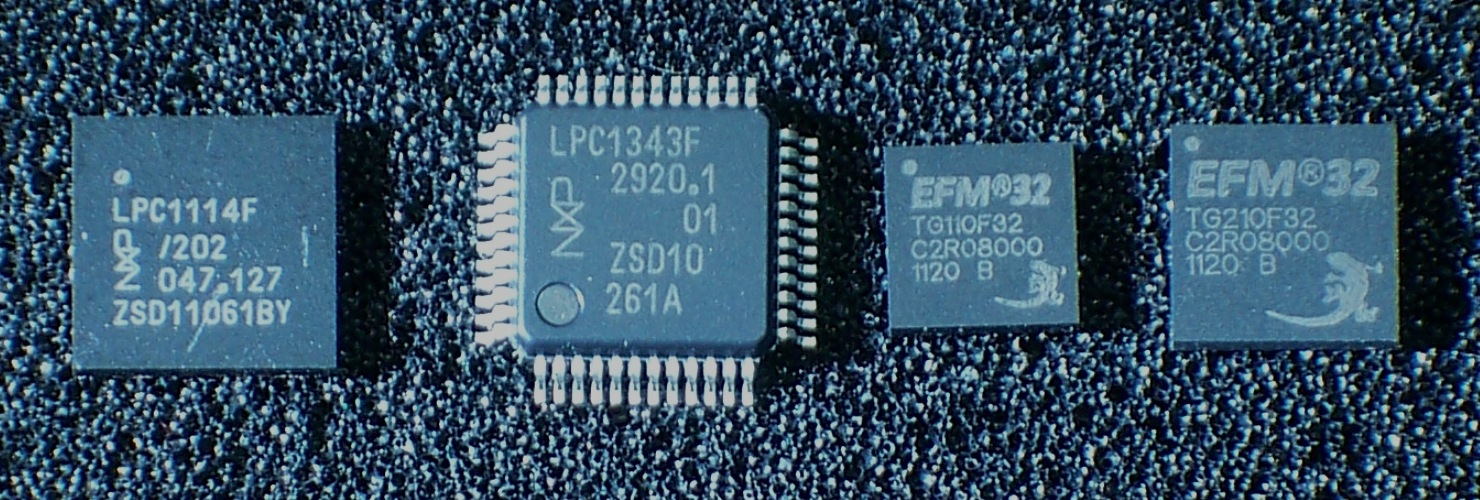
\includegraphics[width=0.65\textwidth, keepaspectratio]{imatges/ARM_Cortex-M0}
 \caption{Diferents microcontrolador Cortex-M0 i M3}{Diferents microcontrolador Cortex-M0 i M3. Per Viswesr [CC BY-SA 3.0], de la Wikimedia Commons \url{https://upload.wikimedia.org/wikipedia/commons/thumb/3/3d/ARM_Cortex-M0_and_M3_ICs_in_SMD_Packages.jpg/512px-ARM_Cortex-M0_and_M3_ICs_in_SMD_Packages.jpg}}
 \label{fig:STAsic}
\end{figure}

\begin{figure}
 \centering
 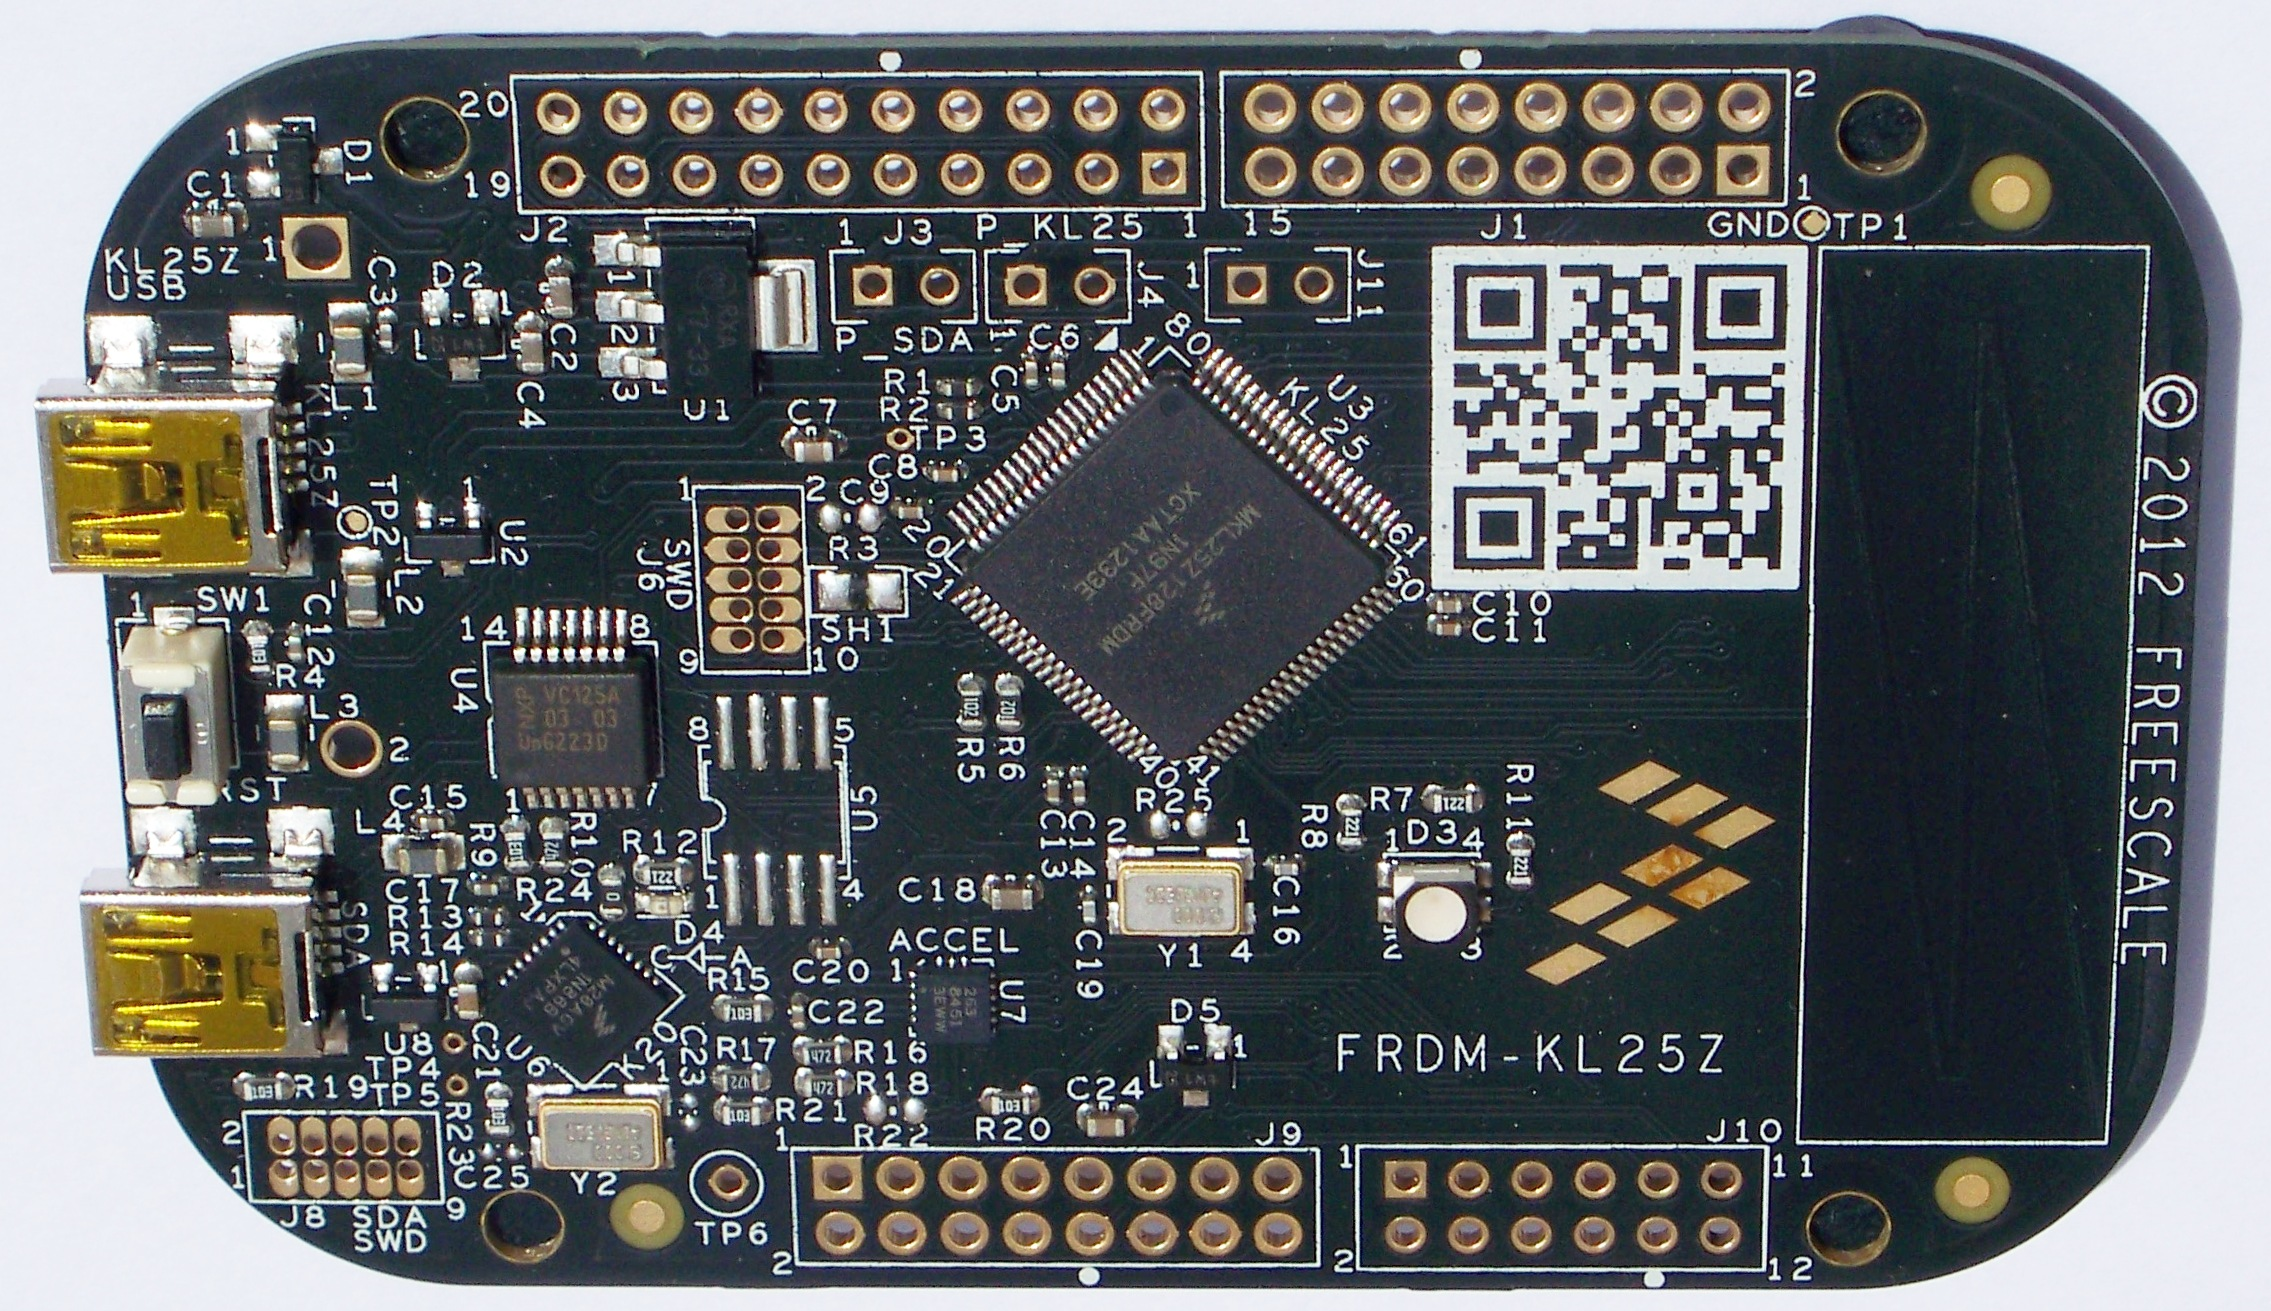
\includegraphics[width=0.65\textwidth, keepaspectratio]{imatges/Freescale_FRDM-KL25Z}
 \caption{Placa Freescale FRDM-KL25Z amb un Cortex-M0+}{Placa Freescale FRDM-KL25Z amb un Cortex-M0+. Per Viswesr [CC BY-SA 3.0], de la Wikimedia Commons \url{https://commons.wikimedia.org/wiki/File:Freescale_FRDM-KL25Z_board_with_KL25Z128VLK_(ARM_Cortex-M0\%2B_MCU).JPG}}
 \label{fig:FRDM}
\end{figure}


\section{Arquitectura}
\label{se:arquitectura}
L'arquitectura dels processadors Cortex-M varia segons la família que estudiem. La família Corte-M0+ té una arquitectura Von Newmann i la resta de famílies tenen arquitectura Harvard mixta, on tot i que la CPU té busos separats per accedir a l'espai de dades o a l'espai de codi, estan tots dos connectats a una sola matriu (Figura~\ref{fig:M3MemoryMap}) \cite[794]{GuideCortexM3M4}.

A part de la CPU pròpiament dita, el que se'n diu {\em core} en els microcontroladors ARM inclou també un controlador d'interrupcions (veure~\fullref{ch:IRQ}), un {\em timer} simple (\fullref{sec:systick}) i un mòdul opcional de protecció de memòria (MPU) \cite[230]{GuideCortexM3M4}. Al ser dispositius comuns a tots els {\em Cores}, l'accés a ells és molt similar entre diferents fabricants (veure \fullref{sec:CMSIS-Core}).

\subsection{Perifèrics mapats a memòria}
\label{sub:memory-mapped}
A l'arquitectura Cortex els perifèrics estan mapats a memòria (\gls{memory mapped}). Això fa que tinguem accessibles els registres de cada perifèric a una regió de memòria determinada. Així doncs, per accedir als registres d'un perifèric per configurar-lo o accedir a les seves dades el que caldrà fer és accedir a una certa adreça de memòria de la forma habitual i llegir o escriure la dada que pertoqui. Aquest mapa de memòria depèn de cada fabricant i model.

\begin{figure}
 \centering
 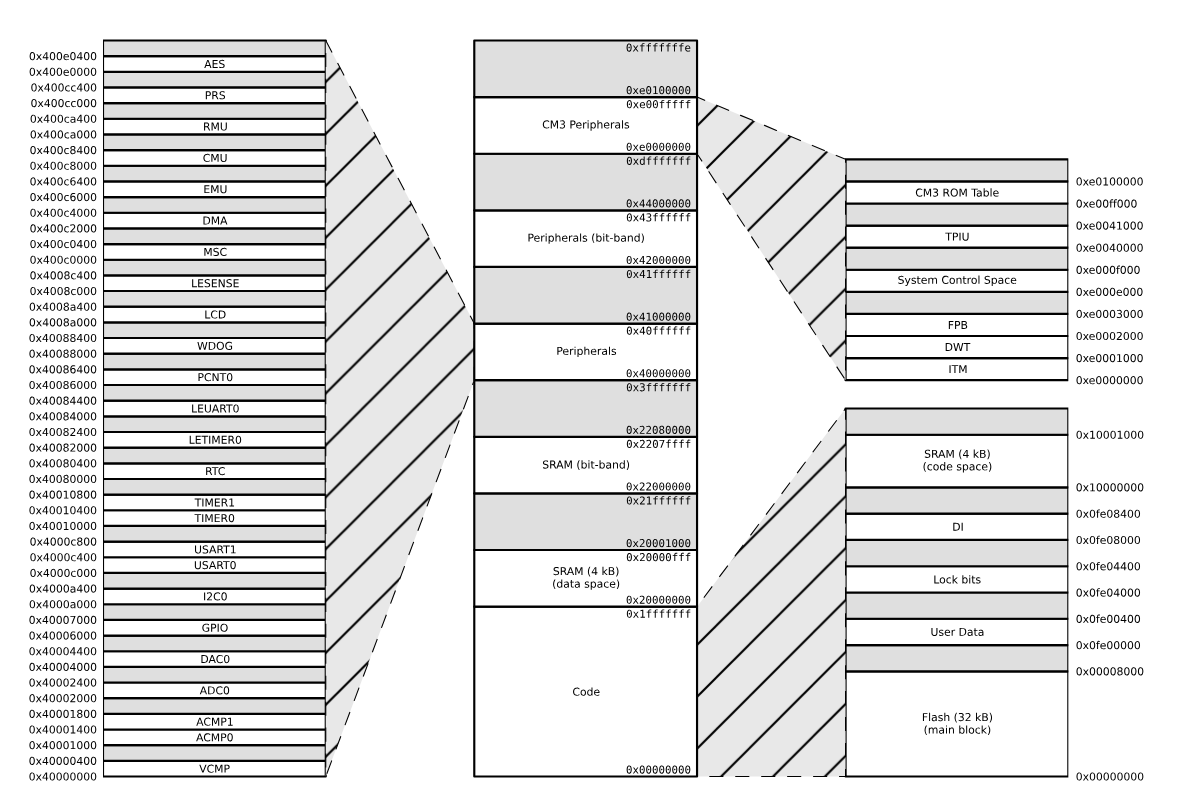
\includegraphics[width=0.85\textwidth, keepaspectratio]{imatges/Cortex-M3-MemoryMap.png}
 \caption{Mapa de memòria d'un Cortex-M3}{Mapa de memòria d'un Cortex-M3 (EFM32TG Reference Manual \cite{EFM32GRM} \copyright SiliconLabs)}
 \label{fig:M3MemoryMap}
\end{figure}

Per exemple, en el Cortex-M3 de la nostra placa, el mapa de memòria és el següent (resumit) (Figura~\ref{fig:M3MemoryMap}):
\begin{itemize}
\item de 0x0000\_0000 fins a 0x1FFF\_FFFF: Codi, aquí hi ha mapat la Flash del microprocessador, incloent-hi la memòria de codi principal, i alguna zona tipus FLASH per l’usuari.
\item de 0x2000\_0000 fins 0x2000\_3FFF la memòria RAM del microprocessador.
\item de 0x4000\_0000 fins 0x40FF\_FFFF estan mapats tots els perifèrics que conformen el microcontrolador. Per exemple:
\begin{itemize}
\item 0x4000\_6000 fins 0x4000\_6FFF hi ha el controlador de \gls{GPIO}
\item 0x4000\_2000 fins 0x4000\_2FFF hi ha l’ADC0.
\item 0x4000\_6000 fins 0x4000\_6FFF hi ha el controlador de GPIO
\end{itemize}
\item etc.
\end{itemize}

Dins de la primera zona hi trobem la zona DI ({\em Device Information}) de l'adreça 0x0FE0\_8000 fins a 0x0FE0\_8400. Aquesta zona guarda certs valors únics per a cada dispositiu. En aquest espai, els registres MEM\_INFO\_FLASH, MEM\_INFO\_RAM i PART\_FAMILY els podem llegir fàcilment \cite[24]{EFM32GRM} (Figura~\ref{fig:EFM32_DI}):

\begin{figure}
 \centering
 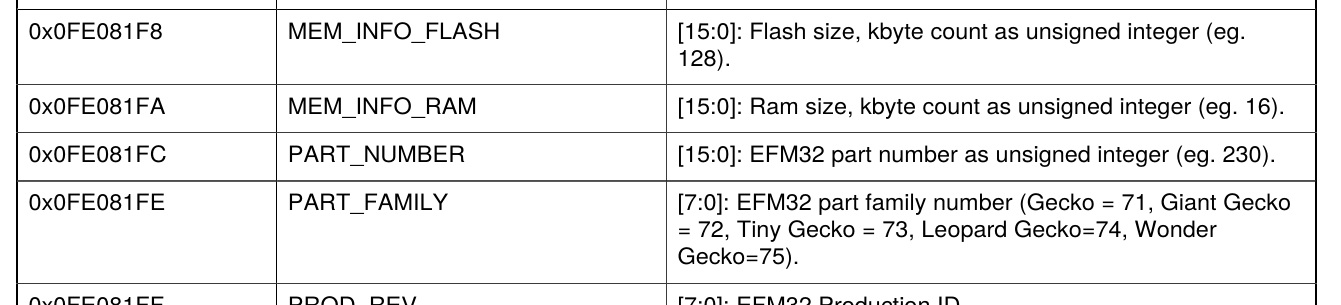
\includegraphics[width=0.85\textwidth, keepaspectratio]{imatges/DI_Table_RM.png}
 \caption{Registres de la DI a usar a l'exemple \cite[24]{EFM32GRM}}
 \label{fig:EFM32_DI}
\end{figure}



\begin{lstlisting}[frame=single,caption={Accedint a memòria en C},label=memorymappedCode,style=customc]
#define FLASH_INFO  (*(unsigned char *)0x0FE081F8)
#define RAM_INFO    (*(unsigned char *)0x0FE081FA)
#define PART_INFO   (*(unsigned char *)0x0FE081FE)

volatile uint32_t aux;

int main(void) {
  while (1) {
    aux = FLASH_INFO; /* 32 kB */
    aux = RAM_INFO;   /* 4 kB */
    aux = PART_INFO;  /* 73 = Tiny Gecko */
  }
}
\end{lstlisting}

Al codi del Llistat~\ref{memorymappedCode} es defineixen les 3 adreces de memòria per ser accedides fent servir un punter. Així, llegint el valor de les definicions FLASH\_INFO, RAM\_INFO o PART\_INFO s'accedeix a la posició de memòria definida de forma directa. Per fer una escriptura es faria igual, però en l'exemple no es pot escriure a cap d'aquests registres. Debugant el codi línia a línia veurem que la variable aux pren el valor corresponent a cada un dels registres mapats.

Enlloc d'accedir a cada registre per separat, com hem fet a l'exemple, es pot definir una estructura que es correspongui amb cada un dels registres d'un perifèric en concret i que aquesta apunti a l'adreça base del perifèric. Així, per accedir a un registre en concret només caldrà accedir al camp de l'estructura definida.

Un exemple d'això el tenim a fitxer efm32g\_devinfo.h, que defineix una estructura d'aquest estil, com es veu al Llistat~\ref {devinfo}.

\begin{lstlisting}[label=devinfo,caption={Exemple de definició d'estructura per accedir a memòria},style=customc]
typedef struct
{
  __IM uint32_t CAL;            /**< Calibration temperature and checksum */
  __IM uint32_t ADC0CAL0;       /**< ADC0 Calibration register 0 */
  __IM uint32_t ADC0CAL1;       /**< ADC0 Calibration register 1 */
  __IM uint32_t ADC0CAL2;       /**< ADC0 Calibration register 2 */
  uint32_t RESERVED0[2];        /**< Reserved */
  __IM uint32_t DAC0CAL0;       /**< DAC calibrartion register 0 */
  __IM uint32_t DAC0CAL1;       /**< DAC calibrartion register 1 */
  __IM uint32_t DAC0CAL2;       /**< DAC calibrartion register 2 */
  __IM uint32_t AUXHFRCOCAL0;   /**< AUXHFRCO calibration register 0 */
  __IM uint32_t AUXHFRCOCAL1;   /**< AUXHFRCO calibration register 1 */
  __IM uint32_t HFRCOCAL0;      /**< HFRCO calibration register 0 */
  __IM uint32_t HFRCOCAL1;      /**< HFRCO calibration register 1 */
  __IM uint32_t MEMINFO;        /**< Memory information */
  uint32_t RESERVED2[2];        /**< Reserved */
  __IM uint32_t UNIQUEL;        /**< Low 32 bits of device unique number */
  __IM uint32_t UNIQUEH;        /**< High 32 bits of device unique number */
  __IM uint32_t MSIZE;          /**< Flash and SRAM Memory size in KiloBytes */
  __IM uint32_t PART;           /**< Part description */
} DEVINFO_TypeDef; /** @} */
\end{lstlisting}

Que es correspon amb els registres de la regió DI a la que hem accedit abans. Aquesta estructura es fa servir al fitxer efm32tg840f32.h definint la referència mostrada al Llistat~\ref {devinfodec}.

\begin{lstlisting}[label=devinfodec,caption={Declaració d'una variable d'accés a la memòria estructurada},style=customc]
#define DEVINFO ((DEVINFO_TypeDef *) DEVINFO_BASE) /**< DEVINFO base ptr */
\end{lstlisting}

De manera que es pot accedir als mateixos registres com s'indica al Llistat~\ref {devinfouse}. Que és una forma bastant més còmoda de treballar.

\begin{lstlisting}[label=devinfouse,caption={Ús de l'estructura d'accés},style=customc]
aux = DEVINFO->MSIZE;
aux = DEVINFO->PART;
\end{lstlisting}

Per sort, la majoria de fabricants proporcionen llibreries de baix nivell que ens estalvien tant conèixer tots els detalls de cada un dels perifèrics com d'haver de manegar els registres un a un: pel cas de SiliconLabs aquestes llibreries s'agrupen sota la EMLIB \cite{EMLIB}; en el cas de l'empresa ST ens proporciona la biblioteca {\em STM32 Standard Peripheral Libraries} \cite{STM32Lib} o la més moderna {\em  STM32Cube hardware abstraction layer (HAL)} \cite{STM32CubeHAL}.

El codi d'aquests exemples està al \href{https://github.com/mariusmm/cursembedded/tree/master/Simplicity/MemoryMap}{repositori del curs}

\subsection{Mida del codi i seccions de memòria}
\label{sub:size}
Quan compilem el nostre codi, com ja sabem, el compilador trasllada el codi C i assemblador a codi màquina, generant un fitxer per cada mòdul que formi l'aplicació (anomenats fitxers objecte amb extensió .o). A continuació el {\em linker} agafa tots els fitxers objecte i crea el fitxer binari tipus ELF.

En aquest fitxer hi ha tota la informació necessària per programar el microcontrolador, i això inclou el codi màquina que cal executar, les definicions de les variables i la seva inicialització, el codi d'inicialització (veure \fullref{sub:boot}), etc. Aquest fitxer serà el que després el programador o {\em debugger} llegirà per tal de programar el microcontrolador.

D'aquest fitxer podem extreure informació valuosa, com és la quantitat de memòria FLASH o RAM que necessita el nostre programa. Això ens ho diu la comanda {\em size} (en el cas del compilador \gls{GCC} per \gls{ARM} la comanda és {\em arm-none-eabi-size}) quan s'executa sobre el fitxer binari creat. La sortida d'aquest programa té el següent aspecte:

\begin{lstlisting}
text    data     bss     dec     hex filename
4976     112      48    5136    1410 SpeedTest_1.axf
\end{lstlisting}

El que està mostrant és la mida (en bytes) de cada un dels segments en que es divideix la nostra aplicació:
\begin{itemize}
 \item {\bf text}: aquest sector és el corresponent al codi executable i les constants definides; també s'inclouen aquí els vectors d'interrupció (veure \fullref{ch:IRQ}). El {\em debugger} s'encarregarà de gravar a la FLASH aquesta secció.
 \item {\bf data}: s'emmagatzemem les dades inicialitzades, com són variables han d'anar a RAM, però també cal guardar el seu valor a la FLASH, per tant, ocupen espai a totes dues memòries. El procés de {\em boot} (Veure \fullref{sub:boot}) copiarà els valors d'inicialització de la FLASH cap a la variable a la RAM.
 \item {\bf bss}: conté totes les variables no inicialitzades. Aquesta secció va a la RAM. Al procés de {\em boot} (Veure \fullref{sub:boot}) aquesta secció s'inicialitza amb zeros.
 \item {\bf dec}: és la suma dels 3 camps anteriors
 \item {\bf hex}: és el mateix valor que {\bf dec} però expressat en hexadecimal.
\end{itemize}

\subsection{Procés de {\em boot}}
\label{sub:boot}
El procés de {\em boot} és tota la seqüència de passes que fa un microcontrolador des de que s'engega fins que comença a executar la nostra funció principal {\bf main()}\index{main()}.

Quan el microcontrolador surt de l'estat de {\em reset} després d'un {\em power-up}, d'un {\em reset} extern, d'un {\em reset} pel Watchdog (veure~\fullref{sec:Watchdog}), etc. cal que s'inicialitzin un seguit de mòduls i peces abans no es pugui començar a executar el nostre codi.

A la posició de memòria 0x0000\_0000 el que hi ha és el vector d'interrupció corresponent al {\em reset} que normalment crida la funció {\bf SystemInit()}\index{SystemInit()} que inicialitza, si cal, parts crítiques del microcontrolador, com el rellotge principal. A continuació es copien les variables inicialitzades de la FLASH a la RAM (secció {\bf data}), s'inicialitza a 0 la secció coneguda com {\bf bss} i per últim crida a la funció {\bf \_start()}\index{\_start()} que acabarà cridant a la nostra funció {\bf main()}\index{main()} \cite{StartUp}. Tot això ho maneguen les eines de forma automàtica i no cal que nosaltres en tinguem cura, però va bé saber què està passant dins el microcontrolador en tot moment.


\section{Rapidesa d'un microcontrolador}
\label{sub:speedtest}
Molts cops no ens fem a la idea de com de ràpid és la CPU d’un microcontrolador. Estem acostumats a llegir i escoltar freqüències de funcionament dels microprocessadors d'escriptori o de servidor, que actualment són de Gigahertz i els nostres pobres microcontroladors van, en el millor dels casos, a uns quants pocs Megahertz. Això ens pot fer pensar que els nostres microcontroladors són lents i que no poden fer gaire coses.

Podem comprovar-ho empíricament.

A l'\href{https://github.com/mariusmm/cursembedded/tree/master/Simplicity/SpeedTest_1}{exemple SpeedTest\_1} hi ha un codi molt simple que simplement incrementa un comptador mentre es té premut el botó 0 i tot seguit imprimeix per la consola el valor al que ha arribat el comptador.
\index{main()}
\begin{lstlisting}[style=customc,caption=Codi velocitat d'un microcontrolador,label=cpuspeed]
void main() {
  ...
  /* while button 0 is pressed, CPU is counting */
  while (GPIO_PinInGet(gpioPortD, 8) == 0) {
    i++;
  }

  if (i != 0) {
    printf("i = %d\n", i); i = 0;
  }
  ...
}
\end{lstlisting}

Això ens hauria de donar una idea de com de ràpid és capaç la nostra CPU de fer operacions aritmètiques simples.

Pitjant el botó molt ràpidament el comptador arriba a 8.000 i 9.000. Així que sembla que compta molt ràpid!

\subsection{Millor mesura de temps}
\label{sub:speedtest_example}
El \href{https://github.com/mariusmm/cursembedded/tree/master/Simplicity/SpeedTest_2}{segon exemple} és una mica més complicat. Per tal de mesurar el temps que es pitja el botó, farem servir un {\em Timer}, que ja ho veurem més endavant (veure \fullref{sub:Timers}). El que es fa a l'exemple és mesurar acuradament el temps que està el botó pitjat i calcular el nombre d'operacions que s'ha fet en aquell temps.

Com podem veure a la Taula~\ref{tb:SpeedTest} el nombre d'operacions per segon es manté constant independentment del temps que estiguem pitjant el botó i és un número força alt, 134.000 sumes per segon!!!

\begin{table}[t!]
\caption{Mesures de temps i sumes per segon}
\centering
\begin{tabular}{|r|c|c|c|c|}
\hline
{\bf Count} & {\bf Ticks (del Timer)} & {\bf Temps (segons)} & {\bf Count/Tick} & {\bf Count/Segon}\\
\hline
16629 & 1688 & 0,12 & 9,85 & 134.677\\
\hline
10955 & 1112	& 0,08 &	9,85	& 134.681\\
\hline
81813 & 8309	& 0,61 &	9,85	& 134.609\\
\hline
17985 & 1826 & 0,13 & 9,85 &134.651 \\
\hline
12054 &1224 & 0,09 & 9,85 & 134.653\\
\hline
269785 &27400 & 2,00 & 9,85 & 134.607\\
\hline
\end{tabular}
\label{tb:SpeedTest}
\end{table}
